\documentclass{article}
\usepackage{cancel}
\usepackage[utf8]{inputenc}
\usepackage {titlesec}
\usepackage[english,russian]{babel}
\usepackage{graphicx}
\usepackage{amssymb}
\graphicspath{{pictures/}}
\usepackage{amsmath}
\titlespacing*{\section}{\parindent}{*4}{*4}
	
	\title{Домашнее задание 5}
	\author{Ткачев Андрей, группа 166}
	\date{\today}

\begin{document}
	\maketitle
	
	\section{Задача 1}
	Любое дерево - связанный граф без циклов, а значит не содержит циклов нечетной длины $\Rightarrow$ любое дерево - двудольный граф. 
		
	В двудольном графе можно выделить как минимум два независимых множества - собственно доли графа, суммарное число вершин в которых равно числу вершин в графе. Но тогда в дереве на $2n$ вершин можно выделить одно независимое множество в котором не меньше половины вершин в силу принципа Дирихле.
	
	\section{Задача 2}
	Пусть в дереве $n$ вершин, степень ни одной из которых не степени 2. Среди этих вершин - $x$ висячих, степень которых по определению равна 1. Тогда $deg$ оставшихся $n - x$ вершин не меньше $3 - x$. Тогда, если сумма всех степеней в графе $D$, то
	$$ D \geqslant x  + 3(n - x)$$
	
	Но по лемме о рукопожатиях $D = 2|E| = 2(n - 1)$ т.к. в дереве число ребер на 1 меньше числа вершин. Получаем неравенство:
	
	$$ 2(n - 1) \geqslant -2x + 3n$$
	$$ 2x \geqslant n + 2$$
	$$ x \geqslant \frac{n}{2} + 1$$
	
	Что и является требуемой оценкой.
	
	\section{Задача 4}
	
	Рассмотрим граф, в котором $(n - 2)^3$ вершины соответствуют кубикам внутреннего под-куба $(n - 2) \times (n - 2) \times (n - 2)$ и еще одна вершина $u$ соответствует всем крайним кубикам куба. Вершины соединены ребром если и только если из соответствующих им кубиков можно перейти друг в друга сломав только одну перегородку (соответственно с $u$ соединим те вершины, кубики которых имеют общую грань с внешней стеной).
	
	Поймем, что любой путь в этом графе однозначно задает способ сломать перегородки соответствующие ребрам так, чтобы все кубики из этого пути были достижимы друг из друга или из каких-то барьерных элементов при разрушение тех самых перегородок. 
	
	Тогда, остовное дерево этого графа задает способ сломать перегородки так, что бы число разрушений было минимально, и при этом всегда существовал путь к от любого кубика к границе, ведь число ребер остова графа $G$ фиксировано и является минимальным допустимым для сохранения связанности при удалении ребер $G$, а раз в дереве все вершины соединены путем с $u$, то все кубики при таких разрушениях имеют доступ к границе.
	
	Таким образом достаточно удалить всего лишь $|E| = ((n - 2)^3 + 1) - 1$ перегородок.
	
	\textbf{Ответ:} $(n - 2)^3$ 
	
	\section{Задача 5}
	
	Рассмотрим граф, вершинами которого являются цифры $0 .. 9$. Соединим ориентированным ребром две вершины если они образуют число кратное 7 в порядке, заданном направлением стрелки, т.е. одно из чисел \linebreak
	$14, 21, 28, 35, 42, 49, 56, 63, 70, 84, 91, 98$:
	
	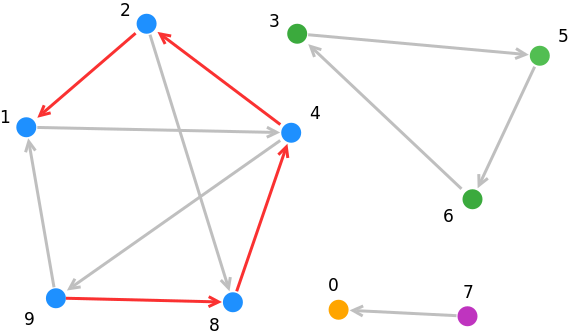
\includegraphics[scale=0.6]{5_1}
	
	Поймем, что числа в которых подряд стоящие цифры образуют кратные 7 двузначные числа и все цифры различны получаются простым обходом каких-то вершин в данном графе. Но поймем тогда, что самый длинный простой путь в этом графе состоит из вершин $9, 8, 4, 2, 1$. Значит число 98421 - самое большое из удовлетворяющих условию: оно во-первых - самое длинное (пятизначное), а во-вторых содержит все цифры самой большой из компонент связанности, причем поставленные в порядке убывания.
	
	\textbf{Ответ:} 98421.
	
	\section{Задача 6}
	Выделим в графе какое-нибудь остовное дерево и рассмотрим какой либо простой путь в этом дереве, начинающийся в одном листе $u$, и заканчивающийся в другом листе $v$ (В любом дереве хотя бы 2 листа, и любой путь из одной вершины в другую - простой). Зададим ориентацию на ребрах этого пути в направлении обхода.
	
	
\includegraphics[scale=0.6]{6_1}
	
	Рассмотрим теперь все вершины, которые в остове соединены с вершинами пути. Ориентируем эти вершины по направлению к вершинам пути. 
	
	Если в остове еще остались вершины, не соединенные ориентированным ребром с уже существующим ориентированным подграфом, то выделим из них те, которые связаны ребром с вершинами из ориентированного подграфа, и зададим направление к нему. Будем повторять до тех пор, пока в остове не останется вершин не связанных с ориентированным подграфом ориентированным ребром (Число вершин конечно, а на каждой итерации мы уменьшаем число вершин вне ориентированной конструкции). 
	
	Заметим, что по построению на каждой итерации мы получаем такой ориентированный подграф, в котором из любой вершины можно добраться в  $v$.
	
	Это можно доказать по индукции по номеру итерации. "После n итераций мы получим ориентированный граф в котором из все вершин достигается $v$". 
	
	База: итерация 1 - в пути из $u$ в $v$ можно было добраться от любой вершины до $v$, значит при указанной ориентации соединенных с путем вершин мы добавили к конструкции некоторое число вершин из которых можно дойти до главного пути, а по нему в $v$. 
	
	Тогда пусть верно для итерации n. Поймем, что на итерации n + 1 мы задаем ориентацию ребер остова в направлении уже существующего подграфа, а значит из всех новых вершин мы можем добраться до $v$ по предположению. Значит верно для всех $n$.
	
	\section{Задача 7}
	
	Докажем, что в турнире на $n$ вершинах всегда есть Гамильтонов путь по индукции по числу вершин.
	
	База $n=1$. Очевидно есть Гамильтонов путь.
	
	Предположение. Пусть верно, что в турнире на $n=k, k>2$ вершинах есть Гамильтонов путь.
	
	Шаг индукции. Рассмотрим граф турнир на $n=k + 1$ вершинах. Зафиксируем вершину $k + 1$. По предположению индукции оставшиеся $k$ соединены Гамильтоновым путем. Пронумеруем вершины этого пути от 1 до $k$. Тогда рассмотрим такую вершину $i$ этого пути которая имеет максимальный индекс, и из которой ведет ребро в нашу фиксированную вершину $k + 1$. 
\begin{center}
	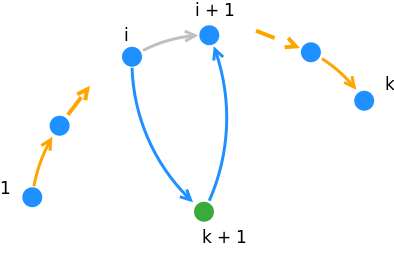
\includegraphics[scale=0.5]{7_1}
\end{center}
	Раз $i$ максимальна, то во все вершины начиная с $i + 1$ ребро идет из $k + 1$. Тогда рассмотрим путь $$0 \longrightarrow 1 \longrightarrow ... i \longrightarrow k + 1 \longrightarrow i + 1 \longrightarrow ... k$$
	
	Поймем, что этот путь Гамильтонов: он проходит через все $k + 1$ вершины. Тогда на всем множестве натуральных чисел верно, что в турнире с $n$ вершинами есть г. путь.
	
	\section{Задача 8}
	
	Возьмем какую-нибудь вершину $u \in V$. Она соединена ровно с $n - 2$ вершинами направленным исходящем ребром и не соединена исходящим ребром ровно с одной вершиной $v$.
	
	\subsection{I}
	Есть ребро из $v$ в $u$. Рассмотрим тогда множество $N(u)$ ориентированных соседей $u$ (т.е. те в которые есть ребро из $u$). Поймем, что из любой $w \in N(u)$ есть ребро ведущее либо в $u$ либо в $v$, либо в обе вершины сразу.
	
	Если $\forall w \in N(u)$ нет исходящего ребра в $v$, то в графе всего 2 компоненты связанности: вершина $v$, которая не достижима из остальных и все оставшиеся вершины, которые очевидно взаимно достижимы. 
	\begin{center}
		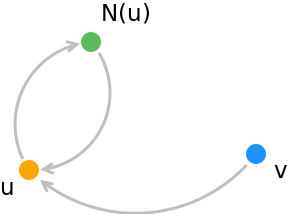
\includegraphics[scale=0.5]{8_1}
	\end{center}
	
	
	Иначе, есть хоть одна $w$ из $N(u)$ из которой есть ребро в $v$. Но тогда граф сильно связанный: из $u$ можно достигнуть соседей $u$, из соседей $u$ можно достигнуть либо $v$, либо саму $u$, а из $v$ есть ребро в $u$.
	
		\begin{center}
			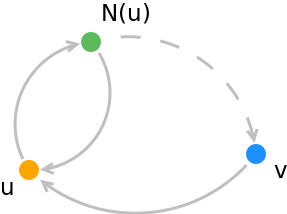
\includegraphics[scale=0.5]{8_2}
		\end{center}
	
	\subsection{II}
	
	Если из $v$ нет ребра в $u$, то из $u$ и из $v$ дуги идут к одним и тем же $n - 2$ вершинам, образующих множество $N$. $\forall w \in N$ обязательно соединена либо с $u$, либо с $v$, или с обоими, т.к. $|N \setminus \{w\}| = n - 3$, а $d(w) = n - 2$.
	
	Поймем, что если $\exists w' \in N $ из которой есть путь в $u$ и если $\exists w'' \in N $ из которой есть путь в $v$, то граф сильно связный: из $u$ можно прийти во все вершины, из которых достижима $v$, а из $v$ во все вершины из которых достижима $u$ - все эти категории в совокупности покрывают все вершины. 
	
		\begin{center}
			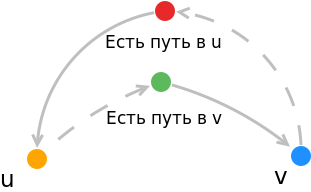
\includegraphics[scale=0.5]{8_3}
		\end{center}	
	
	Иначе, все вершины из $N$ ведут только в одну из вершин $u$ или $v$. Не вредя общности, будем считать, что все дуги из $N$ ведут в $u$. Но тогда все вершины из $N + \{u\}$ взаимно достижимы, а $v$ не достижима ни от куда.
		\begin{center}
			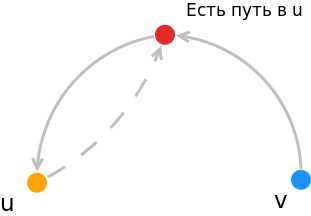
\includegraphics[scale=0.5]{8_4}
		\end{center}
	
	\textbf{Ответ:} Одна или две компоненты связанности равновероятно. 
	 
	
\end{document}